\documentclass[a4paper]{report}
\usepackage[toc,page]{appendix}
\usepackage[english]{babel}
\usepackage[utf8]{inputenc}
\usepackage{amsmath}
\usepackage{float}
\usepackage{graphicx}
\usepackage[colorinlistoftodos]{todonotes}
\usepackage[nottoc]{tocbibind}

\usepackage{listings}

\definecolor{dkgreen}{rgb}{0,0.6,0}
\definecolor{gray}{rgb}{0.5,0.5,0.5}
\definecolor{mauve}{rgb}{0.58,0,0.82}

\lstset{frame=tb,
  language=Python,
  aboveskip=3mm,
  belowskip=3mm,
  showstringspaces=false,
  columns=flexible,
  basicstyle={\small\ttfamily},
  numbers=none,
  numberstyle=\tiny\color{gray},
  keywordstyle=\color{blue},
  commentstyle=\color{dkgreen},
  stringstyle=\color{mauve},
  breaklines=true,
  breakatwhitespace=true,
  tabsize=3,
  escapeinside=||
}


\title{Theme D Experiment for fluid dynamics \& Incubation of coastal ecosystem}

\author{Thumwanit Napat Group 2 \\ 16B00133}

\date{\today}
\begin{document}
\nocite{*}
\maketitle

\chapter{Experiment for fluid dynamics}
\label{sec:firstExperiment}

\section{Background \& Theories}
The setting and knowledge are based on the handout of the experiment, Theme D.

The experiment was splitted into 3 sections. The first part is preparatory experiment for measure the
based value for the next section. The second section is for simultaing the situation where there is a blockage which disturb the
flow. The last section simulate the situation where the ground is filled by coral which slow down the flow.
\begin{enumerate}
    \item {\bf Flow rate} - Derived from Bernoulli's equation
    \begin{equation}\label{eq:flow_rate}
        q_1=\sqrt{2gh_1^2(h_0-h_1)}=C_ca\sqrt{2g(h_0-C_ca)} \ \ \left(C_c=\frac{h}{a}\right)    
    \end{equation}
    
    
    \item {\bf Froude number \& Energy loss} - 
    By conservation of energy, energy loss from hydraulic jump can be formulated as the following.
    \begin{equation}\label{eq:enegy}
        \Delta E = \frac{(h_2-h_1)^3}{4h_1h_2} \ \ (h_2 > h_1)
    \end{equation}

    By the conservation of momentum, ratio of $h_1$ and $h_2$ can be expressed and rewritten as the following formular
    \begin{equation}\label{eq:froude}
        \frac{h_2}{h_1}=\frac{1}{2}\left[\sqrt{1+8F_{r_1}^2}-1\right]
    \end{equation}
    
    \item {\bf Drag force} - Drag force inflicted by the impact of the fluid can be expressed as the following
    \begin{equation}\label{eq:drag}
        F_D=\frac{1}{2}\rho C_DAU^2
    \end{equation}
    where $C_D$, $A$, $U$ are the drag coefficient, projected area and flow velocity accordingly.
    
\end{enumerate}

\section{Result}
\subsection{Preparatory Experiment}
\begin{table}[H]
    \centering
    \begin{tabular}{|c|c|}\hline
        Dimension & Value \\\hline
        $h_0$ & 15 cm \\\hline
        $h_1$ & 1 cm \\\hline
        $h_2$ & 1.2 cm \\\hline
        $W$ (Width of the channel) & 38.3 cm \\\hline
        $W_\text{internal}$ (Width of the channel) & 38.3 cm \\\hline
        $L$ (Length of the channel) & 2.48 m \\\hline
        $a$ (height of the gate) & 1 cm \\\hline
    \end{tabular}
    \caption{list of the dimension of channel and height of water level}
    \label{tb:prep_list}
\end{table}

\begin{table}[H]
    \centering
    \begin{tabular}{|c|c|}\hline
        Number of measurements & Time (second) \\\hline
        1 & 7.76 \\\hline
        2 & 7.27 \\\hline
        3 & 7.43 \\\hline
    \end{tabular}
    \caption{value of time (s) to fill the bucket (8 L)}
    \label{tb:prep_time}
\end{table}

\subsection{Hydraulic jump test}
\begin{table}[H]
    \centering
    \begin{tabular}{|c|c|}\hline
        Dimension & Value \\\hline
        $h_1$ & 0.9 cm \\\hline
        $h_2$ & 4.6 cm \\\hline
    \end{tabular}
    \caption{Hydraulic jump test measured values}
    \label{tb:jump}
\end{table}

\subsection{Drag force test}

\begin{table}[H]
    \centering
    \begin{tabular}{|c|c|}\hline
        Dimension & Value \\\hline
        Width of channel & 38.3 cm \\\hline
        Diameter of cylinder & 8.9 cm \\\hline
        $M_1$ (mass of cylinder in the case without porous bed) & 9.7 cm \\\hline
        $M_2$ (mass of cylinder in the case with porous bed) & 88 gm \\\hline
        $h_3$  (in the case without porous bed) & 1.5 cm \\\hline
        $L$ (Length of the channel) & 2.48 m \\\hline
        $a$ (height of the gate) & 1 cm \\\hline
    \end{tabular}
    \caption{list of the dimension of channel and height of water level}
    \label{tb:drag}
\end{table}

\section{Discussion}

\subsection{Contraction coefficient and flow rate per unit width}
From equation (\ref{eq:flow_rate}) and information in table \ref{tb:prep_list}, we calculate the contraction coefficient as the following.

\[C_c=\frac{h_1}{a}=\frac{1}{1}=1\]

then calculate the flow rate per unit width

\[q_1=C_ca\sqrt{2g(h_0-C_a a)}=1\times10^{-2}\times\sqrt{2\times9.81\times(15\times10^{-2}-1\times10^{-2})}=1.66\times10^{-2}\frac{\text{m}^2}{\text{s}}\]

From the bucket filling time in table \ref{tb:prep_time}, the average time of filling 8 L of water is $22.46/3=7.49$ s. Therefore, the flow rate Q is

\[Q=\frac{8\times10^{-3}}{7.49}\frac{\text{m}^3}{\text{s}}\]

So that the experimental flow rate per unit width

\[q=\frac{Q}{w_{\text{internal}}}=\frac{8\times10^{-3}}{7.49}\times\frac{1}{10.3\times10^{-2}}\frac{m^3}{s}=1.04\times10^{-2}\frac{m^2}{s}\]

The experimental value is smaller than the theoretical value which might be caused by friction and energy loss.

\subsection{Energy dissipated owing to the hydraulic jump and Froude numbers (Fr)}
We set up the obstacle and measure the height of the water at each point as recorded in the table \ref{tb:jump}. From the equation \ref{eq:enegy}, we can calculate the energy dissipated by hydraulic jump as the following.

\[\Delta E = \frac{\left(h_2-h_1\right)^3}{4h_1h_2}=\frac{\left(4.6-0.9\right)^3}{4\times0.9\times4.6}\text{cm}=3.06\text{cm}\]

And from equation \ref{eq:froude}, we can calculate the froude number ($F_r$) as the following

\[F_{r_1}=\sqrt{\frac{\left(\displaystyle\frac{2h_2}{h_1}+1\right)^2-1}{8}}=3.95\]

Conversely, $F_{r_2}$ can be calculated as the following

\[F_{r_2}=\sqrt{\frac{\left(\displaystyle\frac{2h_1}{h_2}+1\right)^2-1}{8}}=0.34\]

\subsection{Drag Force}
From table \ref{tb:drag} and flow rate ($Q$) from previous section, we obtain the mean velocity as the following

\[\overline{U}=\frac{Q}{h_3\times w}=\frac{8\times 10 ^ {-3}}{7.49}\frac{1}{1.2\times10^{-2}\times38.3\times10^{-2}}=2.32\times10^{-1}\frac{\text{m}}{\text{s}}\]

From equation \ref{eq:drag}, we obtain drag force
\begin{align*}
    \text{Without porous bed } &: \ F_D=\frac{1}{2}\rho C_DA\overline{U}^2= \frac{1}{2}\rho C_D(h_3D)\overline{U}^2=2.26\times10^{-2}\text{N} \\
    \text{With porous bed } &: \ F_D=\frac{1}{2}\rho C_DA\overline{U}^2= \frac{1}{2}\rho C_D(h_3D)\overline{U}^2=5.28\times10^{-2}\text{N}
\end{align*}

From the experimental data, we obtain friction coefficient by balancing the weight and calculate by the following equation,
\begin{align*}
    F_D &= F_R \\
    &= \mu(mg-B)\\
    &=\mu(mg-\rho_{\text{water}}v_{\text{sub}}g)\\
    \mu &=\frac{F_D}{mg-\rho_{\text{water}}v_{\text{sub}}g}
\end{align*}
where $v_{\text{sub}}$ is the volume of the cylinder under the water surface.

\begin{table}[H]
    \centering
    \begin{tabular}{|c|c|c|}\hline
        & Without porous bed & With porous bed \\\hline
        Drag force & $2.26\times10^{-2}$ & $5.28\times10^{-2}$ \\\hline
        Buoyancy force & $4.58\times10^{-1}$ & $1.07$ \\\hline
        Friction coefficient & $1.81\times10^{-2}$ & $-2.55\times10^{-1}$\\\hline
    \end{tabular}
    \caption{Drag force, Buoyancy force and calculated friction coefficient}
    \label{tb:drag-b-mu}
\end{table}

We can observe that the friction coefficient for the case with porous bed became negative. It might be because we assumed that both cases conserve same flow rate which it should decrease by porous bed and force acting on the cylinder also.


\chapter{Incubation of coastal ecosystem}
\label{sec:secondExperiment}

In this experiment, we will measure the photosynthesis and calcification rate of the coral regarding to
the intensity of the light in order to estimate the real world situation of coral reef accumulation. The experiment
was conducted on different intensities, 100\%, 50\%, 25\% and 0\%.

\section{Result \& Discussion}

\begin{table}[H]
\centering
\begin{tabular}{|c|c|c|c|c|c|c|c|c|}
\hline
Time  & Beaker \# & pH    & Beaker \# & w0      & w1      & w2       & pHa   & Intensity \\ \hline
14:10 & 14        & 7.985 & 19        & 44.2417 & 93.4206 & 108.3132 & 3.515 & 100\%     \\ \hline
14:40 & 17        & 8.072 & 15        & 44.3308 & 97.70   & 112.62   & 3.723 & 100\%     \\ \hline
14:50 & 16        & 7.902 & 14        & 44.6421 & 94.4369 & 109.2862 & 3.553 & 50\%      \\ \hline
15:20 & 12        & 7.977 & 15        & 44.3301 & 96.6465 & 111.4785 & 3.681 & 50\%      \\ \hline
15:30 & 13        & 7.818 & 18        & 45.1818 & 97.3689 & 112.1726 & 3.692 & 25\%      \\ \hline
16:00 & 14        & 7.868 & 12        & 45.6516 & 97.6967 & 112.5688 & 3.667 & 25\%      \\ \hline
16:10 & 18        & 7.75  & 11        & 44.0117 & 94.7432 & 109.6703 & 3.591 & 0\%       \\ \hline
16:40 & 19        & 7.722 & 16        & 43.4848 & 95.6989 & 110.5581 & 3.685 & 0\%       \\ \hline
\end{tabular}
\caption{Experimental values}
\label{tab:exp2_value}
\end{table}

\begin{enumerate}
    \item From the table \ref{tab:exp2_value}, we calculate according to the equations in the handout and obtain the following result
    
    \begin{align*}
        G &= -\frac{1}{2}\rho_w\frac{V}{A}\frac{\Delta A_T}{\Delta t} \\
        P_n &= -\rho_w\frac{V}{A}\frac{\Delta C_T}{\Delta t} - G
    \end{align*}
    
\begin{table}[H]
\centering
\begin{tabular}{|c|c|c|c|}
\hline
Time  & Beaker \# & G (mmol/m$^2$h)                           & P (mmol/m$^2$h)                     \\ \hline
14:10 & 14        & {1.431398231}  & {12.4}  \\ \cline{1-2}
14:40 & 17        &                               &                        \\ \hline
14:50 & 16        & {1.324916993}  & {9.86}  \\ \cline{1-2}
15:20 & 12        &                               &                        \\ \hline
15:30 & 13        & {0.2226796472} & {5.43}  \\ \cline{1-2}
16:00 & 14        &                               &                        \\ \hline
16:10 & 18        & {0.214260976}  & {-2.46} \\ \cline{1-2}
16:40 & 19        &                               &                        \\ \hline
\end{tabular}
\caption{P and G experimental values}
\label{tab:PG_value}
\end{table}
    
    \item Using non-linear least square fitting, the result was obtained as the following graph and equation.
    \begin{table}[H]
        \centering
        \begin{tabular}{|c|c|c|c|}\hline
            E & $P_{observe}$ & $P_{model}$ & $(P_{observe} - P_{model})^2$ \\\hline
            440 & 12.4 & 12.44 & 2.32$\times 10^{-3}$ \\\hline
            250 & 9.86 & 9.7 & 1.65$\times 10^{-2}$ \\\hline
            135.8 & 5.43 & 5.54 & 1.12$\times 10^{-2}$ \\\hline
            0.4 & -2.4 & -2.49 & 6.63$\times 10^{-4}$ \\\hline
            \multicolumn{1}{c}{} & \multicolumn{1}{c|}{} & sum & 3.078$\times 10^{-2}$ \\\cline{3-4}
        \end{tabular}
        \caption{experimental and predicted P error table}
        \label{tab:my_label}
    \end{table}

\begin{figure}[H]
    \centering
    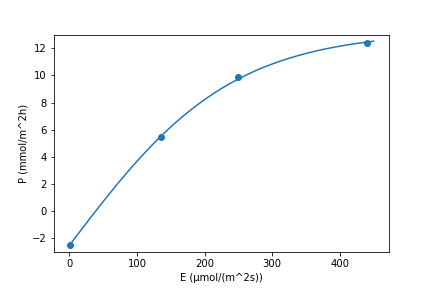
\includegraphics{E-P.png}
    \caption{E-P Graph}
    \label{fig:my_label}
\end{figure}

\[P = 15.8\tanh{\left(\frac{E}{2.40\times 10^2}\right)} - 2.51\]

\item Analogously, We obtain the graph and equation for G.

    \begin{table}[H]
        \centering
        \begin{tabular}{|c|c|c|c|}\hline
            E & $G_{observe}$ & $G_{model}$ & $(G_{observe} - G_{model})^2$ \\\hline
            440 & 1.431 & 1.496 & 4.151$\times 10^{-3}$ \\\hline
            250 & 1.325 & 1.004 & 1.028$\times 10^{-1}$ \\\hline
            135.8 & 0.2223 & 0.6102 & 1.502$\times 10^{-1}$ \\\hline
            0.4 & 0.2143 & 0.08287 & 1.726$\times 10^{-2}$ \\\hline
            \multicolumn{1}{c}{} & \multicolumn{1}{c|}{} & sum & 2.744$\times 10^{-1}$ \\\cline{3-4}
        \end{tabular}
        \caption{experimental and predicted G error table}
        \label{tab:my_label}
    \end{table}

\begin{figure}[H]
    \centering
    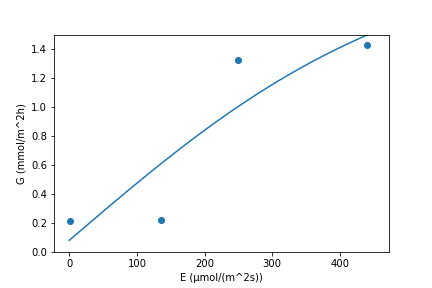
\includegraphics{E-G.png}
    \caption{E-G Graph}
    \label{fig:my_label}
\end{figure}

\[G = 2.016\tanh{\left(\frac{E}{5.056\times 10^2}\right)} + 8.128\times 10^{-2}\]

\item The calcification rate per day of a coral community can be estimated by integrating the calcification rate of a whole day

\begin{equation}
    rate = coverage \times \int^{24}_{0} G(t) dt \ ;\  t \text{ is in hour}
\end{equation}
where $E_b$ was derived as the following equation (From top to bottom)
\begin{align*}
G &= 2.016\tanh{\left(\frac{E_b}{5.056\times 10^2}\right)} + 8.128\times 10^{-2}\\
    E_b &= E_s(1-\alpha)\exp(-\lambda h) \\
    E_s &= 2.1\times Q\\
    Q &= \max \left(\frac{S\cos^2Z}{(\cos Z+2.7)e\times10^{-5}+1.085\cos Z+0.10}, 0\right)\\
    \cos Z &= \sin\phi\sin\Delta + \cos\phi\cos\Delta\cos HA\\
    \Delta &= 23.44^{\circ}\times\cos[(172-D)\times2\pi/365]\\
    HA &= (12 - t) \times \pi / 12
\end{align*}

With the following constants
\begin{align*}
    coverage &= 0.3\\
    h &= 0.5 \ \text{m}\\
    \phi &= 20^{\circ}\text{N}\\
    D &= 71 (\text{March 21})\\
    e &= 1783\\
    \alpha &= 0.07\\
    \lambda &= 0.12\ \text{m}^{-1}
\end{align*}

The implementation was done by Python which the code was attached in the Appendix. Then we plot the graph of $G$.

\begin{figure}[H]
    \centering
    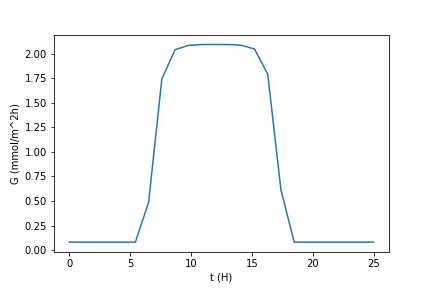
\includegraphics{G4-t.png}
    \caption{G vs time in March $21^{\text{st}}$}
    \label{fig:my_label}
\end{figure}

By utilizing simpson method to do integration, we yield the following result

\begin{equation}
    rate = coverage \times \int^{24}_{0} G(t) dt = 6.571 \ \text{mmol}/\text{m}^2\text{day}
\end{equation}

\item
In this question, assume that calcium carbonate (CaCO$_3$) molar weighted 100 g mol$^{-1}$ and 1.4 g cm$^{-3}$ of bulk density of the reef. By these factor, we can calculate the accumulation rate as the following

\begin{align*}
    \text{accumulation rate} &= \frac{6.571\times10^{-7}\ \text{mol}/\text{cm}^2\text{day}\times100\ \text{g mol}^{-1}}{1.4\ \text{g cm}^{-3}}\times365\ \text{day/year}\\
    &= 0.1713 \ \text{cm/year}
\end{align*}

\item Sea level rise 0.5 cm/year while the accumulation of coral reef per year is 0.1713 cm. Therefore, for keeping the coastal protection efficiency, the necessary coverage of the coral is
\[coverage_{\text{new}} = coverage_{\text{prev}}\times0.5 / 0.1713=0.8757\]

or 87.57\% coverage required. 
There are many factors that damaging the coral reef site such as physical damage, from divers, trashes or irresponsible boat. If the diver touch the coral, it may stir up the sediment and cause damage to the coral which education toward tourism should be strengthen. The indirect way is chemical from household or waste water. Another important factor is CO$_2$. As the result of increase of CO$_2$, the rate of calcification decrease and the accumulation of coral reef become slower. To solve these problems, we need to reduce our usage of energy, decrease the CO$_2$ emission, and use less water to reduce the waste water which will return to the ocean eventually.

\end{enumerate}

\begin{appendices}
\begin{lstlisting}[caption={Q4 code snippet for calculating $E_b(t)$},captionpos=b]
S = 1353
phi = 20 * (2 * np.pi / 360)
delta = 23.44 * np.cos((172 - 71) * 2 * np.pi / 365) * (2 * np.pi / 360)
alpha = 0.07
lmbda = 0.12
h = 0.5
e = 1783
cover = 0.3

def max0(x):
    return (x > 0) * x 

def Q(cosz):
    return max0(S * cosz ** 2 / ((cosz + 2.7)*e*10**-5+1.085*cosz+0.1))

def cosz(HA):
    return np.sin(phi) * np.sin(delta) + np.cos(phi) * np.cos(delta) * np.cos(HA)

def HA(t):
    return (12 - t) * np.pi / 12.

def Es(Q):
    return 2.1 * Q

def Eb(Es):
    return Es * (1 - alpha) * np.exp(-lmbda * h)

# Eb input by t (time)
def Eb_a(t):
    HA_t = HA(t)
    cosz_t = cosz(HA_t)
    Q_t = Q(cosz_t)
    Es_t = Es(Q_t)
    return Eb(Es_t)
\end{lstlisting}
\end{appendices}

\bibliographystyle{unsrt}
\bibliography{sample}

\end{document}